\section{Applications}
\label{sec:app}
% Blaze is originally designed for quantum simulation to make the code more readable and extensible while perserving the performance of hand-optimized parallel code.
% We achieved this by adapt our quantum simulation algorithm into a series of MapReduce operations and create a highly optimized MapReduce implementation.

% We find that our implentation can also be useful for many data mining tasks as well, because many data mining tasks share the same kind of MapReduce workflows as our quantum simulation algorithm and our implementation can allow us to write more concise and extensible code with the high-level MapReduce API while achieving the performance of hand-optimized parallel C++ code.
In this section, we benchmark Blaze against a popular data mining package Spark, on common data mining tasks, including word frequency count, PageRank, k-means, expectation maximization (with the Gaussian Mixture model), and k-nearest neighbors search.

\subsection{Task Description and Implementation}

In this section, we describe the data mining tasks and how we implement them in Blaze and Spark.
All the source code of our implementation is included in our GitHub repository~\cite{blaze}.

\subsubsection{Word Frequency Count}

This task counts the number of occurrences of each unique English words in a text file.
We use the Bible and Shakespeare's works as the testing text.
Since Spark has significant overhead in starting the MapReduce tasks, we repeat the Bible and the Shakespeare 200 times, so that the input file contains about 0.4 billion words.

We use MapReduce in both Blaze and Spark.
The mapper function takes a single line and emits multiple (word, 1) pairs.
The reducer function sums the values.
Appendix \ref{app:wordcount} contains the full Blaze implementation for this example.

\subsubsection{PageRank}

This task calculates the PageRank score, which is defined as the stationary value of the following equation:
\begin{equation}
    \label{eq:pr}
    PR(p_i) = \frac{1-d}{N} + d \sum_{p_j\in M(p_i)} \frac{PR(p_j)}{L(p_j)}
\end{equation}
where $M(p_i)$ is the set of pages that link to $p_i$, $L(p_j)$ is the number of outbound links from page $p_j$, $N$ is the total number of pages, and $d=0.15$.
When a page has no outbound links, it is called a sink and is assumed to connect to all the pages.
We use the graph500 generator to generate the input graph which contains 10 million links.
We set the convergence criterion to $10^{-5}$, which results in 27 iterations for our input.
The links are stored distributedly across multiple machines.

For Blaze, we use 3 MapReduce operations per iteration to implement this task.
The first one calculates the total score of all the sinks.
The second one calculates the new PageRank scores according to Eq.~\ref{eq:pr}.
The third one calculates the maximum change in the scores of all the pages.
For Spark, we use the built-in PageRank module from the Spark GraphX library~\cite{xin2013graphx}.

\subsubsection{K-Means}

K-Means is a popular clustering algorithm.
The algorithm proceeds by alternating two steps until the convergence.
The first step is the assignment step where each point is assigned to the nearest clustering center.
The second step is the refinement step where each clustering center is updated based on the new mean of the points assigned to the clustering center.

We generate 100 million random points around 5 clustering centers as the testing data, and use the same initial model and convergence criteria for Spark and Blaze.
The points are stored distributedly across multiple machines.

For Blaze, we use a single MapReduce operation to perform the assignment step.
The update step is implemented in serial.
For Spark, we use the built-in implementation from the Spark MLlib library~\cite{meng2016mllib}.

\subsubsection{Expectation Maximization}

This task uses the expectation maximization method to train the Gaussian Mixture clustering model (GMM).
Starting from an initial model, we first calculate the Gaussian probability density of each point for each Gaussian component
\begin{equation}
    \label{eq:prob}
    p _{ k } \left( \vec{ x } | \theta _{ k } \right) = \frac{ 1 }{ \left( 2 \pi \right) ^{ d / 2 } \left| \Sigma _{ k } \right| ^{ 1 / 2 } } e ^{ - \frac{ 1 }{ 2 } \left( \vec{ x } - \vec{ \mu } _{ k } \right) ^{ T } \Sigma _{ k } ^{ - 1 } \left( \vec{ x } - \vec{ \mu } _{ k } \right) }
\end{equation}
where $\mu_1$ to $\mu_K$ are the centers of these Gaussian components and $\Sigma_1$ to $\Sigma_K$ are the covariance matrices.
Then we calculate the membership of each point for each Gaussian component
\begin{equation}
    \label{eq:membership}
    w _{ i k } = \frac{ p _{ k } \left( \vec{ x } _{ i } | \theta _{ k } \right) \cdot \alpha _{ k } }{ \sum _{ m = 1 } ^{ K } p _{ m } \left( \vec{ x } _{ i } | \theta _{ m } \right) \cdot \alpha _{ m } }
\end{equation}
where $\alpha_k$ is the weights of the Gaussian component.
Next, we calculate the sum of membership weights for each Gaussian component $N_k=\Sigma_{i=1}^K w_{ik}$.
After that, we update the parameters of the Gaussian mixtures
\begin{align}
    \alpha _{ k } ^{ } =& \frac{ N _{ k } }{ N }\\
    \label{eq:mu}
    \vec{ \mu } _{ k } =& \left( \frac{ 1 }{ N _{ k } } \right) \sum _{ i = 1 } ^{ N } w _{ i k } \vec{ x } _{ i }\\
    \label{eq:sigma}
    \Sigma _{ k } =& \left( \frac{ 1 }{ N _{ k } } \right) \sum _{ i = 1 } ^{ K } w _{ i k } \left( \vec{ x } - \vec{ \mu } _{ k } \right) ^{ T } \left( \vec{ x } - \vec{ \mu } _{ k } \right)
\end{align}
Finally, we calculate the log-likelihood of the current model for these points to determine whether the process is converged.
\begin{equation}
    \label{eq:log}
    \sum _{ i = 1 } ^{ N } \log p \left( \vec{ x } _{ i } | \Theta \right) = \sum _{ i = 1 } ^{ N } \left( \log \sum _{ k = 1 } ^{ K } \alpha _{ k } p _{ k } \left( \vec{ x } _{ i } | \theta _{ k } \right) \right)
\end{equation}

We generate 1 million random points around 5 clustering centers as the testing data and use the same initial model and convergence criteria for Spark and Blaze.
The points are stored distributedly across multiple machines.

For Blaze, we implement this algorithm with 6 MapReduce operations per iteration.
The first MapReduce calculates the probability density according to Eq.~\ref{eq:prob}.
The second MapReduce calculates the membership according to Eq.~\ref{eq:membership}.
The third MapReduce accumulates the sum of memberships for each Gaussian component $N_k$.
The next two MapReduce perform the summations in Eq.~\ref{eq:mu} and Eq.~\ref{eq:sigma}.
The last MapReduce calculates the log-likelihood according to Eq.~\ref{eq:log}.
For Spark, we use the built-in implementation from the Spark MLlib library~\cite{meng2016mllib}.

\subsubsection{Nearest 100 Neighbors}

In this task, we find the 100-nearest neighbors of a point from a huge set of other points.
This is a common procedure in data analysis and recommendation systems.
We use 200 million random points for this test.

For both Spark and Blaze, we implement this task with the \emph{top k} function of the corresponding distributed containers and provide custom comparison functions to determine the relative priority of two points based on the Euclidean-distance.

\subsection{Performance Analysis}

We test the performance of both Spark and Blaze for the above tasks on Amazon Web Services (AWS).
The time for loading data from the file system is not included in our measurements.
Spark is explicitly set to use the \lstinline{MEMORY_ONLY} mode and we choose memory-optimized instances r5.xlarge as our testing environments which have large enough memory for Spark to complete our tasks.
Each r5.xlarge has 4 logical cores, 32GB memory, and up to 10 Gbps network performance.
% It is based on Intel Xeon Platinum 8000 series (Skylake-SP) processors with a sustained all core Turbo CPU clock speed of up to 3.1 GHz.

For Spark, we use the AWS Elastic MapReduce (EMR) service version 5.20.0 , which comes with Spark 2.4.0.
Since in the default setting, Spark changes the number of executors on the fly, which may obscure the results, we set the environment variable for maximizing resource allocation to true to avoid the change.
We also manually specify the number of partitions to 100 to force the cross-executor shuffle on the entire cluster.
For Blaze, we use GCC 7.3 with -O3 optimization and MPICH 3.2. 
% We also test the effects of using Thread-Caching Malloc (TCMalloc) from Google, the results of which are indicated by Blaze TCM.
For both Spark and Blaze, we perform warmup runs before counting the timings.
Timings are converted to more meaningful results for each task.

% We test Spark and Blaze on the five tasks mentioned above, which are word frequency count (Worldcount), PageRank, K-Means, Expectation Maximization (EM GMM) and Nearest 100 Neighbors (NN100) Search.
The detailed performance comparison are shown in Fig.~\ref{fig:wordcount_speed} to \ref{fig:nn}.
% ``\textbf{Spark}'', ``\textbf{Spark (MLlib)}'', ``\textbf{Spark (GraphX)}'', ``\textbf{Blaze}'', ``\textbf{Blaze TCM}''
``Spark'', ``Spark (MLlib)'', ``Spark (GraphX)'', ``Blaze'', ``Blaze TCM'' denote the original Spark implementation, the MLlib library in Spark, the GraphX library in Spark, original Blaze, and Blaze linked with Thread-Caching Malloc (TCMalloc), respectively.

As shown in Fig.~\ref{fig:wordcount_speed} to \ref{fig:nn}, Blaze outperforms Spark significantly on all five data mining applications.
On average, Blaze is more than 10 times faster than Spark.
The superior performance of Blaze shows that our highly-optimized implementation suits these data mining applications well.
The performance difference between Blaze and Blaze TCM is negligible.
However, without using TCMalloc, the performance has more fluctuations and can occasionally experience a significant drop of up to 30\%.
% For specific applications, Blaze achieves at least $4 \times$ higher performance in K-Means, while it achieves $40 \times$ higher performance in PageRank.

\begin{figure}
  \begin{center}
  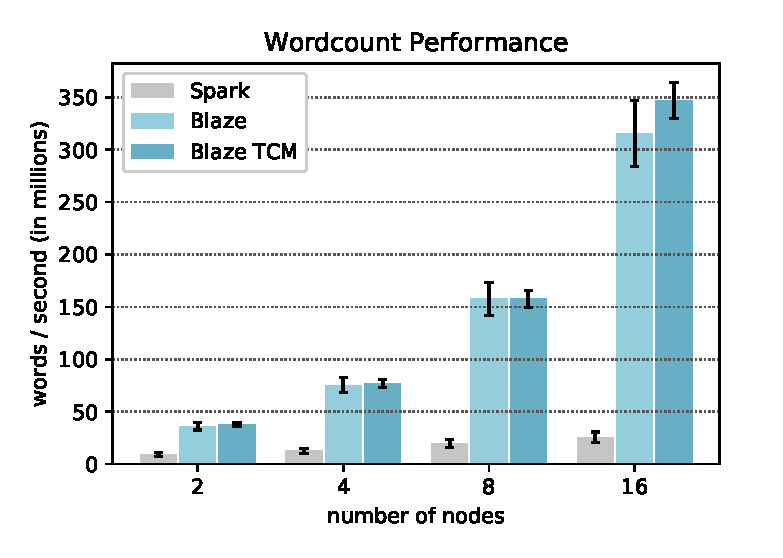
\includegraphics[width=\linewidth]{wordcount_speed.eps}
  \end{center}
  \vspace{-0.2cm}
  \caption{Performance of the word frequency count measured in the number of words processed per second.
%   For Spark, we use the example code from its official website.
%   For Blaze, we implement the algorithm with 1 MapReduce operation.
  }
  \label{fig:wordcount_speed}
\end{figure}
\begin{figure}
  \begin{center}
  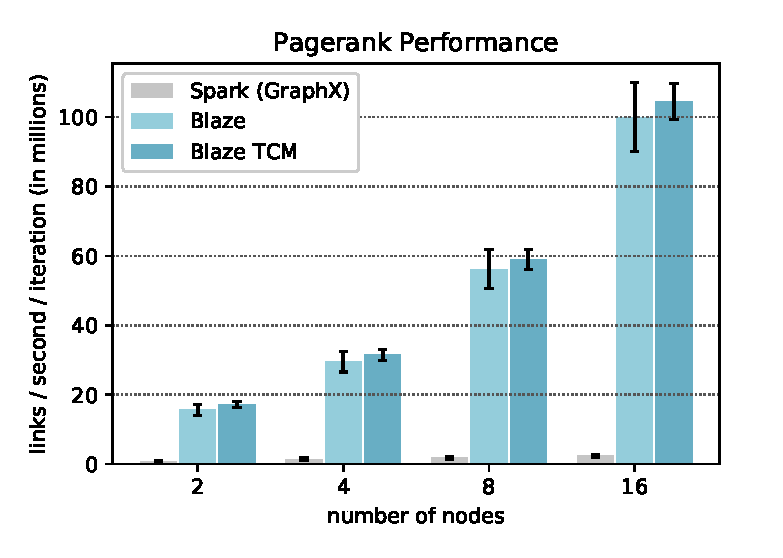
\includegraphics[width=\linewidth]{pagerank_speed.eps}
  \end{center}
  \vspace{-0.2cm}
  \caption{Performance of the PageRank algorithm measured in number of links processed per second per iteration.
%   For Spark, we use the built-in implementation from its GraphX library.
%   For Blaze, we implement the algorithm with 2 MapReduce operations per iteration.
  }
  \label{fig:pagerank_speed}
\end{figure}
\begin{figure}
  \begin{center}
  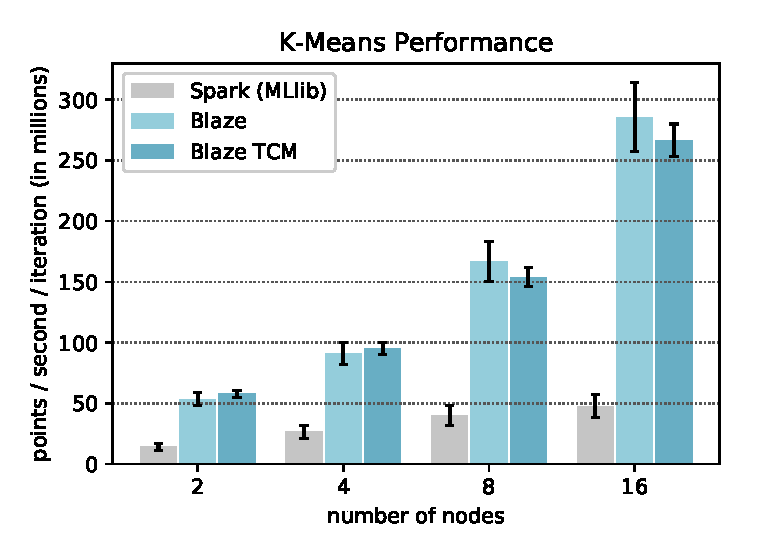
\includegraphics[width=\linewidth]{kmeans_speed.eps}
  \end{center}
  \vspace{-0.2cm}
  \caption{Performance of the K-Means algorithm measured in the number of points processed per second per iteration.
%   For Spark, we use the built-in implementation from its MLlib library.
%   For Blaze, we implement the algorithm with 1 MapReduce operation per iteration.
  }
  \label{fig:kmeans_speed}
\end{figure}
\begin{figure}
  \begin{center}
  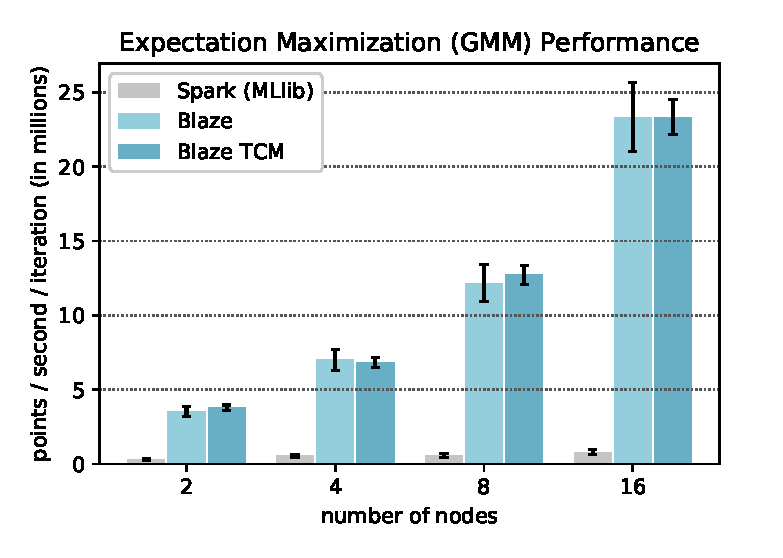
\includegraphics[width=\linewidth]{em_speed.eps}
  \end{center}
  \vspace{-0.2cm}
  \caption{Performance of the Expectation Maximization algorithm for the Gaussian Mixture Model measured in the number of points processed per second per iteration.
%   For Spark, we use the built-in implementation from its MLlib library.
%   For Blaze, we implement the algorithm with 6 MapReduce operations per iteration.
  }
  \label{fig:em}
\end{figure}
\begin{figure}
  \begin{center}
  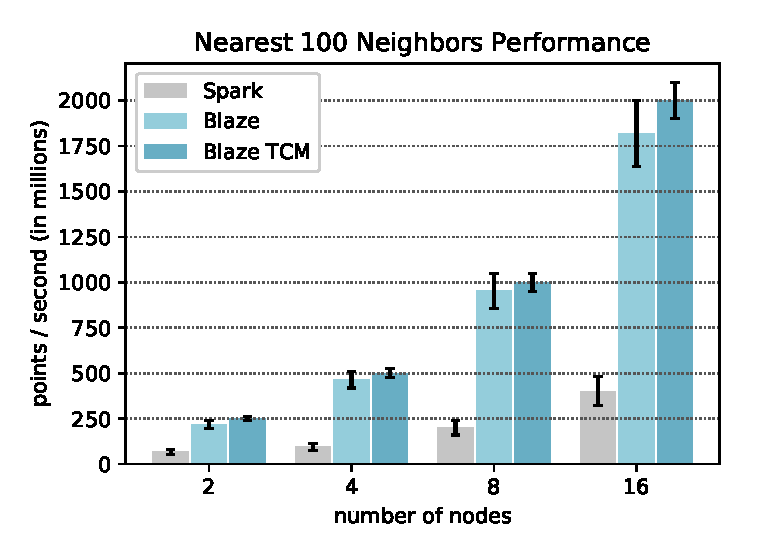
\includegraphics[width=\linewidth]{nn_speed.eps}
  \end{center}
  \vspace{-0.2cm}
  \caption{Performance of the Nearest 100 Neighbors search measured in the number of total points processed per second.
%   For both Spark and Blaze, we use the top function with a custom compare function.
  }
  \label{fig:nn}
\end{figure}
\subsection{Memory Consumption}

We measure the memory consumption for running these tasks on a single local machine of 12 logical cores, using the same versions for all the software as the tests on AWS.
As shown in Fig~\ref{fig:mem}, we can see that both Blaze and Blaze TCM consumes much smaller amount of memory than Spark during the runs, especially for PageRank, K-Means, and expectation maximization (GMM), where Spark uses 10 times more memory than Blaze.
The only case where the memory consumption between Spark and Blaze is close is the k-nearest neighbors search, which does not involve intermediate key/value pairs.

The memory consumption between Blaze and Blaze TCM are always on the same order of magnitude, although in one case, Blaze consumes 40\% more memory when linked against TCMalloc.

\begin{figure}
  \begin{center}
  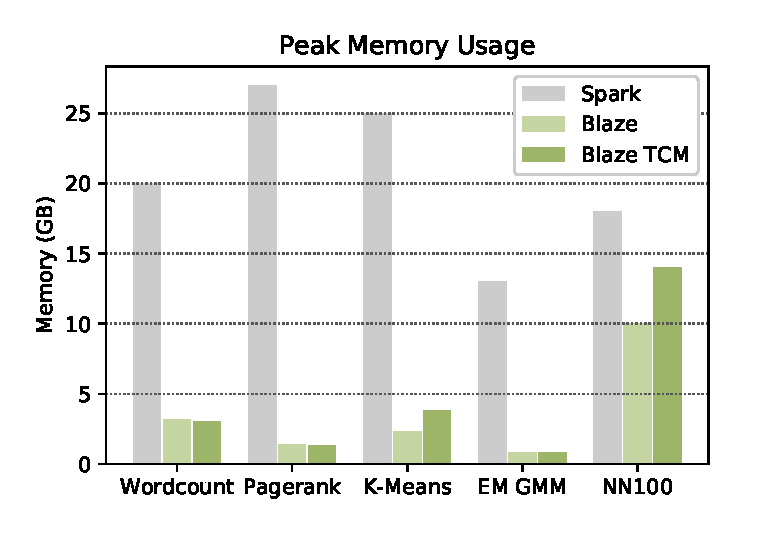
\includegraphics[width=1.0\linewidth]{memory.eps}
  \end{center}
  \vspace{-0.5cm}
  \caption{Peak memory usage on a single node.
%   of 12 logical cores and 64GB memory.
%   Word frequency count task processes 350 millions words.
%   Pagerank task processes 10 million links iteratively.
%   K-means task processes 100 million points iteratively.
%   Expectation maximization (Gaussian Mixture Model) task processes 1 million points iteratively.
%   Nearest 100 neighbors task searches the nearest neighbors from 200 million points.
  }
  \label{fig:mem}
\end{figure}

\subsection{Cognitive Load}

Cognitive load refers to the efforts needed to develop or understand the code.
Minimizing the cognitive load is the ultimate goal that MapReduce and its variants try to achieve.

There are lots of different measures for cognitive efforts.
Source lines of code is not a good measure here as Spark/Scala supports chaining functions and can put several consecutive operations on a single line.
Hence, a line of Spark/Scala may be much more difficult to understand than a line of C++.
Here we use the number of distinct APIs used as the indicator for cognitive load.
It is a legitimate indicator because people will have to do more searches and remember more APIs when a library requires more distinct API calls to accomplish a task.

Spark's built-in implementation uses about 30 different parallel primitives for different tasks, while Blaze only uses the MapReduce function and less than 5 utility functions.
We can see from Fig.~\ref{fig:cog} that the cognitive load of using Blaze is much smaller than using Spark.

\begin{figure}
  \begin{center}
  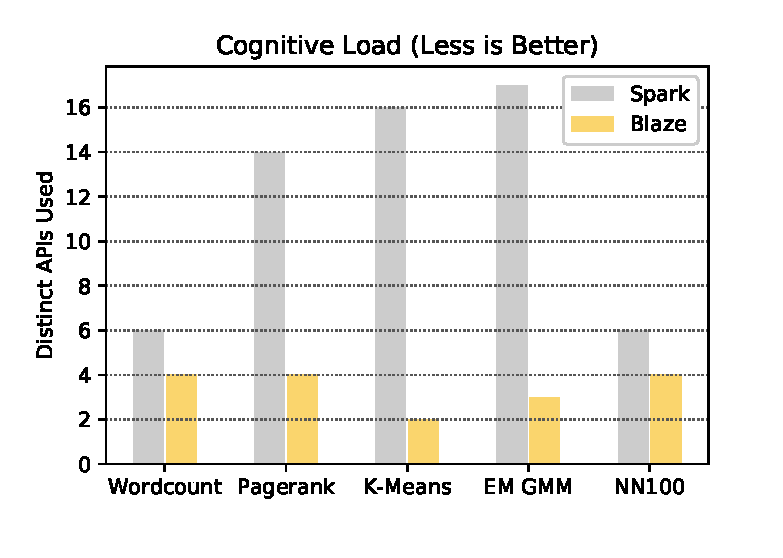
\includegraphics[width=1.0\linewidth]{cognitive.eps}
  \end{center}
  \vspace{-0.5cm}
  \caption{Cognitive load comparison between Blaze and Spark.}
  \label{fig:cog}
\end{figure}